
\section{Calibration par optimisation en boite noire et politique de contrôle\label{sec:odometry_cmaes}}

Cette section décrit les travaux menés en collaboration avec Ludovic Hofer sur
la calibration de l'odométrie prédictive par optimisation en boite noire et 
l'apprentissage d'une politique de déplacement pour le robot Sigmaban.

Afin de répondre aux limitations opérationnelles posées par le 
système de capture de mouvements (voir section \ref{sec:odometry_lwpr_limits_and_conclusions}),
une approche ne nécessitant aucun capteur externe est développée.
Cette approche se base sur la mesure manuelle du déplacement final du robot 
sur plusieurs séquences d'apprentissage ainsi que sur la
calibration d'un modèle de correction linéaire au travers d'une phase d'optimisation.
Cette technique a pu être appliquée avec succès au cours de la compétition 
RoboCup 2016 en Allemagne.

De plus comme proposé dans le paragraphe \ref{sec:odometry_lwpr_limits_and_conclusions}, 
cette section explore l'application de la calibration de l'odométrie prédictive
à la planification du déplacement du robot.
Plus précisément, une politique de contrôle du déplacement du robot 
est développée afin de résoudre le problème de l'approche de la balle.
Cette politique est basée sur le formalisme des processus de décisions markovien 
(\textit{Markov Decision Processes}, MDP) continus à la fois sur l'espace d'actions 
ainsi que sur l'espace des états.\\

Lors d'un match de football robotique, les robots doivent repérer la balle, 
se localiser sur le terrain, être capable de tirer dans la balle et de se relever. 
Mais l'action la plus couteuse en temps et potentiellement source de gains importants
est l'approche de la balle. Après sa détection, le robot commence par 
se diriger vers la balle à vitesse maximale.
Il doit ensuite se positionner avec précision
afin de placer la balle dans une petite zone devant l'un de ses pieds en position de
tir et avec la bonne orientation (face aux buts adverses).
Le fort bruit du déplacement rend cette tâche complexe.
Le temps nécessaire à l'approche de la balle est comparé entre un algorithme 
d'approche expert utilisé lors de l'édition 2016 et l'approche MDP.

Dans cette étude, la méthode de calibration de l'odométrie présentée se concentre
sur l'odométrie prédictive. Cependant et comme démontré dans la section \ref{sec:odometry_lwpr},
la calibration de odométrie proprioceptive se fait se façon très similaire.
Les travaux de Ludovic Hofer sur la planification et le solutionneur MDP 
sont résumés mais non détaillés.
Le lecteur pourra se référer au contenu de l'article publié, \cite{ApproachICAPS2017}, 
ou au document de thèse de Ludovic pour plus d'amples de précisions.

\subsection{Méthodes d'optimisation en boite noire et CMA-ES\label{sec:blackbox}}

Les méthodes d'optimisation en boite noire (\textit{blackbox}) également 
nommées méthodes sans dérivée\footnote{Selon les auteurs, ces deux termes 
ne sont pas exactement équivalents ; un certain flou concernant ce vocabulaire 
reste présent dans la littérature.} (\textit{dervative-free}) représentent un
domaine de recherche très actif dans le monde de l'optimisation.

Le problème est de trouver pour une fonction de $\mathbb{R}^{n} \rightarrow \mathbb{R}$
non linéaire et souvent non convexe
le ou les points de l'espace d'entrée minimisant (ou maximisant) sa valeur
de sortie ; possiblement en respectant un ensemble de contraintes.
L'optimisation analytique manipule les expressions mathématiques du problème
pour en tirer directement la forme close des solutions exactes.
Quand ces problèmes sont mathématiquement trop complexes pour être
manipulés symboliquement, une optimisation numérique et itérative est
alors menée. Ces méthodes se basent sur la connaissance des valeurs 
numériques des dérivées partielles et se résument in fine à une
descente (ou monté) du gradient de la fonction à optimiser.
L'optimisation en boite noire intervient en dernier ressort quand 
il n'est pas possible, trop couteux ou trop bruité d'accéder aux 
dérivées partielles de la fonction.
Quand la forme ou les propriétés de la fonction ne
sont pas connues ou ne peuvent être exploitées.
Au prix d'un temps de convergence parfois bien plus long, il est supposé 
que seule l'évaluation de la fonction est possible.
La performance de ces algorithmes est alors mesuré en 
le nombre d'évaluations nécessaires pour trouver la solution
du problème (à marge d'erreur fixée).

Le développement et l'utilisation de ces méthodes en boite noire 
ont été particulièrement actifs ces vingt dernières années dans
différents domaines de la science et de l'ingénierie.
Typiquement, elles sont particulièrement adaptées à l'optimisation
de systèmes dont le comportement n'est connu qu'au travers de
simulations numériques complexes, sans possibilité d'étude analytique.
En 2009, le premier ouvrage de référence entièrement consacré 
au domaine de l'optimisation sans dérivée est rédigé 
par \cite{conn_introduction_2009}.

Des approches très diverses ont été développées et peuvent être
classées selon différents axes.
Certains algorithmes ont une exploration déterministe alors que
d'autres réalisent un échantillonnage stochastique de la fonction.
Certains exploitent directement les points évalués
alors que d'autres se basent sur la construction d'un modèle de substitution
(\textit{surrogate model}) approximant la fonction recherchée.
Enfin, certains algorithmes se concentrent sur une exploration locale
d'optimum alors que d'autres recherchent un optimum global.
La plupart des méthodes d'optimisation supposent de plus que la fonction 
étudiée soit déterministe et ne présente pas de bruit. 
Dans le cas contraire, d'autres techniques spécifiques ont 
été développées. On peut par exemple évoquer 
\cite{coulom_clop:_2011} et \cite{cauwet_noisy_2016}.

Une comparaison des performances de multiples implémentations
d'optimisation en boite noire disponibles en 2013 est réalisée
par \cite{rios_derivative-free_2013}.
Souvent, les méthodes effectivement implémentées sont hybrides
et empruntent des idées à plusieurs approches.
La non convexité, la taille de la dimension ainsi que la non
régularité (\textit{non-smooth}) de la fonction à optimiser 
sont les principaux facteurs rendant le problème difficile.\\

Dans cette étude, le choix de la méthode d'optimisation en boite noire 
s'est porté sur l'algorithme CMA-ES, \textit{Covariance Matrix Adaptation Evolution Strategy}
ou stratégies d'évolution avec adaptation de la matrice de covariance
présenté par \cite{hansen_completely_2001} et \cite{hansen_cma_2006}.
CMA-ES appartient aux catégories des méthodes stochastiques, 
exploitant directement les évaluations de la fonction et 
recherchant un optimum local.
De la même manière que l'algorithme du recuit simulé s'inspire
d'un processus physique, CMA-ES est un algorithme évolutionniste.

D'après la comparaison de \cite{rios_derivative-free_2013},
CMA-ES se positionne dans le milieu haut du classement des méthodes
d'optimisation en boite noire en 2013.
De plus, il s'avère comparativement plus compétitif sur les
problèmes de plus hautes dimensions et ayant moins de régularité.
Les meilleurs algorithmes sont d'après cette étude les implémentations 
commerciales de TOMLAB en MATLAB.
CMA-ES est cependant l'une des meilleurs méthodes de cette liste
à posséder une implémentation de référence en C++.

L'état de l'algorithme CMA-ES entre chaque itération est représenté par
une distribution normale multivariée.
Sa moyenne représente l'estimation du minimum actuel de la fonction et
sa matrice de covariance la zone d'exploration locale courante.
À chaque itération, un certain nombre fixé de points sont échantillonnés
depuis la distribution puis évalués par la fonction.
Les points sont triés selon leur score et la distribution
est mise à jour afin de maximiser la vraisemblance d'obtenir
de meilleurs scores à la prochaine itération.
L'historique des deux précédentes moyennes est également 
conservée afin de contrôler la longueur du pas d'une manière similaire
à une descente de gradient.
L'algorithme a peu de paramètres principaux\footnote{De nombreux critères 
d'arrêt peuvent cependant intervenir.} : la taille de la population 
(ou nombre d'évaluations par itération), le nombre maximum d'itérations, 
le nombre maximum de redémarrages et optionnellement la variance de l'exploration initiale.
Il est de plus conseillé de normaliser les dimensions d'entrées afin qu'elles
évolues toutes dans les mêmes ordres de grandeurs.

En réalité, de nombreuses variations de l'algorithme CMA-ES existent, 
et notamment en ce qui concerne la politique de redémarrage.
Pour trouver un minimum global d'une fonction fortement non connexe et possédant
de nombreux minimas locaux, il est conseillé de relancer plusieurs fois
l'algorithme (stochastique) avec une configuration initiale différente.
Par exemple en initialisant la recherche avec un autre point de départ 
ou en variant la taille de la population.
Pour être plus précis, la version exacte de CMA-ES employée ici a pour
nom \og \textit{abipop} \fg pour \textit{adaptative bi-population}.
Cette version est présentée par \cite{hansen_benchmarking_2009}.\\

En pratique, nous nous basons sur la bibliothèque logicielle \textit{libcmaes}
(\url{https://github.com/beniz/libcmaes}) implémentée par Emmanuel Benazera 
avec l'aide de Nikolaus Hansen.
Le code est libre, écrit en C++ moderne (C++11) et ne dépend que de
la bibliothèque d'algèbre linéaire \textit{Eigen}.
Elle possède également une interface python et est considérée comme
l'implémentation de référence en C++.
Son grand intérêt est aussi d'implémenter la parallélisation multi-coeur
des évaluations de la fonction réduisant d'autant les temps de calculs.

\subsection{Définition du problème de l'approche}

Comme mentionné précédemment, l'amélioration du contrôle de l'approche 
de la balle est source de gains de temps importants pendant les
matchs de football robotique.
La balle est tout d'abord détectée dans l'image de la caméra 
et sa position est exprimée dans l'espace des pixels.
Le modèle géométrique du robot ainsi que la connaissance
des ouvertures angulaires optiques de la caméra permet alors d'estimer 
sa position cartésienne sur le sol dans le repère égocentrique 
du robot\footnote{Il s'agit de calculs géométriques simples dont l'implémentation
peut être consultée à l'adresse suivante :
\url{https://github.com/RhobanProject/Model/blob/master/Model/HumanoidModel.hpp}.
À noter que la précision de cette estimation est assurée par une 
étape de calibration du modèle de caméra. Cette calibration se base sur une
méthode de maximisation de la log-vraisemblance non présentée dans ce manuscrit.}.

La détection de la balle à lieu tout au long du mouvement à une fréquence au maximum 
aux alentours de $10$ Hertz. 
Cependant, il est courant que la détection échoue ou que la balle soit
perdue de vue pendant plusieurs secondes.
Comme le robot se déplace continuellement, la position de la balle 
n'est pas stockée dans le repère mobile égocentrique du robot mais dans 
le repère du monde lié au modèle géométrique.
Grâce à l'intégration de l'odométrie proprioceptive compensant 
le déplacement du robot, il est ainsi possible de continuer
à asservir le mouvement du robot sur la position de la balle même 
en l'absence de nouvelle observation\footnote{Une gestion des horodatages
permet de plus de compenser de cette manière la latence de traitement
de la vision qui pouvait atteindre en 2016 jusqu'à $300$~ms de retard.}.\\

Malgré ce mécanisme, les erreurs d'intégration de l'odométrie, 
d'estimation de la position de la balle mais surtout les perturbations
du mouvement de marche \textit{IKWalk} rendent l'asservissement 
du déplacement difficile.
Ceci est particulièrement le cas lors du placement final 
à moins d'un mètre de la balle.
De loin, la précision est moins importante que la vitesse de déplacement.
Le robot met en effet plus de temps à bien se placer devant la balle
une fois arrivé à proximité qu'à parcourir en ligne droite la moitié 
du terrain afin de la rejoindre.

Le problème se résume donc de la manière suivante : sachant la position 
de la balle et l'orientation des buts adverses cibles (dans le repère du monde), 
quelle est la séquence d'ordres à envoyer au générateur de marche pour piloter
le robot devant la balle avec l'orientation cible. 
Et ceci, sans entrer en collision avec la balle.
Toucher la balle tend à la faire rouler sur le sol ce qui oblige à
recommencer le placement et fait perdre un temps important à l'approche.\\

\begin{table}[h]
  \caption{\label{table:approach_state_space}Espace d'état de l'approche}
  \centering
  \begin{tabular}{|l|c|c|c|}
    \hline
    Nom & Unité & minimum & maximum\\
    \hline
    Distance à la balle & $m$ & 0 & 1\\
    Direction à la balle & $rad$ & $-\pi$ & $\pi$\\
    Direction de tir & $rad$ & $-\pi$ & $\pi$\\
    Vitesse d'avance (\textit{stepGain}) & $\frac{m}{\mathrm{pas}}$ & -0.02 & 0.04\\
    Vitesse latérale (\textit{lateralGain}) & $\frac{m}{\mathrm{pas}}$ & -0.02 & 0.02\\ 
    Vitesse de rotation (\textit{turnGain}) & $\frac{\mathrm{rad}}{\mathrm{pas}}$ & -0.2 & 0.2\\
    \hline
  \end{tabular}
\end{table}

\begin{table}[h]
  \caption{\label{table:approach_action_space}Espace d'action de l'approche}
  \centering
  \begin{tabular}{|l|c|c|c|}
    \hline
    Nom & Unité & minimum & maximum\\
    \hline
    Accélération d'avance ($\Delta$\textit{stepGain}) & $\frac{m}{\mathrm{pas}^2}$            & -0.02 & 0.02  \\
    Accélération latérale ($\Delta$\textit{lateralGain}) & $\frac{m}{\mathrm{pas}^2}$            & -0.01 & 0.01  \\
    Accélération en rotation ($\Delta$\textit{turnGain}) & $\frac{\mathrm{rad}}{\mathrm{pas}^2}$ & -0.15 & 0.15  \\
    \hline
  \end{tabular}
\end{table}

Afin de limiter les déstabilisations du mouvement de marche, des bornes
sont imposées à la fois sur la vitesse du robot (ordres de la marche) ainsi
que sur son accélération (variations des ordres à chaque cycle de marche).
En conséquence, le contrôle du déplacement du robot s'exerce
au niveau de l'accélération plutôt que de la vitesse.
Ces limites sont détaillées dans les tableaux \ref{table:approach_state_space}
et \ref{table:approach_action_space} listant respectivement
les dimensions de l'espace d'état (informations utilisés à chaque cycle pour 
contrôler le déplacement) et d'action (ordres en accélération de la marche).

On peut remarquer que la vitesse de la balle n'est pas considérée ici.
Premièrement, les oscillations latérales de la tête du robot pendant la marche
sont à l'origine d'un bruit non négligeable sur le calcul de la position cartésienne de la balle.
L'estimation de la vitesse de la balle sur le terrain, alors que le robot lui même se déplace
est un problème difficile.
D'autre part, dans l'état actuel du niveau de jeu du football robotique, 
la balle reste majoritairement immobile.
Les joueurs passant la plus grande partie du temps à atteindre 
la balle et à se positionner.

À noter également que pour simplifier l'apprentissage de la politique de contrôle, 
le pied de support (qui est une variable binaire) n'est pas présent dans l'espace d'état.
Les ordres de la marche ne sont donc mis à jour qu'au début de chaque cycle de marche soit
au début de la phase de support gauche. À chaque cycle, les deux pas consécutifs 
gauche droit exécutent le même déplacement.\\

Lors de l'édition 2015 de la RoboCup, un robot humanoïde expérimental 
de plus grande taille (Grosban, $90$~cm de haut) a été testé.
Il s'est avéré que sur ce robot, les imperfections mécaniques et de contrôle 
moteur étaient démultipliés par rapport à la plateforme Sigmaban en raison
d'un mauvais rapport poids puissance.
Le mouvement de marche s'en est trouvé très affecté et les pas latéraux
quasiment impossibles à stabiliser.
Il pouvait tourner sur lui même, avancer et reculer mais la longueur maximale des
pas chassés était fortement réduite par rapport au robot Sigmaban.
Le mouvement de marche perdait alors une grande partir de sa capacité omnidirectionnelle.
Malheureusement l'approche experte qui se base en grande partie sur les pas 
latéraux pour tourner autour de la balle était alors très inefficace et lente.

C'est pourquoi dans cette étude, les performances de l'approche experte et 
de l'approche par apprentissage sont comparées sur deux types de marches.
La marche normale omnidirectionnelle sur le robot Sigmaban et une
marche quasiment non omnidirectionnelle.
Sur l'approche quasiment non omnidirectionnelle, les bornes de vitesses et d'accélérations
du déplacement latéral sont divisées par $5$ par rapport à leurs valeurs normales
(tableaux \ref{table:approach_state_space} et \ref{table:approach_action_space}).
De même, le bruit latéral de déplacement est également divisé par $2$ (voir plus bas).
Le but est ainsi d'évaluer comparativement la capacité d'adaptation 
de la méthode d'apprentissage à la locomotion de la plateforme robotique.

\subsection{Critères d'évaluation d'une approche\label{sec:odometry_cmaes_fitness}}

Pour évaluer puis comparer en simulation 
la performance de différents algorithmes d'approche, 
$50$ cycles de marche du robot sont simulés.
Après chaque cycle de marche, la pose de la balle dans 
le repère égocentrique du robot est notée par la fonction
de score suivante.
À la fin de la simulation, la somme des scores associés
à chaque cycle de marche quantifie la performance de l'approche 
(le score le plus élevé étant le meilleur) :
\begin{description}
    \item[Zone de tir (0)] : 
        Quand le robot est dans la zone de tir, il reçoit un score nul
        afin d'éliminer les approches ne pouvant pas s'y stabiliser 
        (vitesse trop élevée). 
        La balle doit se trouver entre $0.15$ et $0.20$~m selon
        l'axe égocentrique $\vec{\bm{x}}$, entre $-0.06$ et $0.06$
        selon l'axe $\vec{\bm{y}}$ et la distance angulaire entre 
        la direction de la balle et la direction de tir doit 
        être inférieure à $10$ degrés.
    \item[Zone de collision (-3)] : 
        Quand le robot entre dans la zone de collision autour de
        la position de la balle, il reçoit un score de $-3$.
        Si le robot touche la balle, il tend à la déplacer 
        et à perdre du temps à devoir se replacer.
        La balle ne doit pas de trouver entre $-0.20$ et $0.15$
        selon l'axe égocentrique $\vec{\bm{x}}$ et 
        entre $-0.25$ et $0.25$~m selon l'axe $\vec{\bm{y}}$.
    \item[Éloignement (-100)] : 
        Seule l'approche précise aux alentours de la balle 
        pose problème et est ici étudiée.
        Si l'asservissement du robot fait qu'il s'éloigne à
        plus de $1$~m de la balle, il reçoit une pénalité de 
        $-100$ et la simulation est immédiatement terminée.
    \item[Sinon (-1)] :
        Dans tous les autres cas de déplacement, le robot
        reçoit à chaque cycle de marche un score de -1.
        Les approches atteignant la zone de tir en 
        un nombre minimal de pas sont ainsi préférées.
\end{description}
On peut noter que cette fonction de score est fortement discontinue 
à l'interface de la zone de tir et de la zone de collision.
Cette discontinuité, exprimant le fait que l'objectif à atteindre 
est très proche de la zone à éviter, rend plus difficile la 
convergence des méthodes de planification.

Au début de chaque simulation, la pose du robot 
est aléatoirement initialisée en dehors des 
zones de tir et de collision.
La distance à la balle est uniformément tirée dans
l'intervalle $[0.4,0.95]$ et l'orientation dans $[-\pi,\pi]$.

Enfin, après chaque cycle de marche simulé, des perturbations 
stochastiques sont ajoutées au déplacement du robot toujours
dans son repère égocentrique.
En translation sur les axes $\vec{\bm{x}}$ et $\vec{\bm{y}}$,
un bruit uniforme tiré entre $-0.02$ et $0.02$~m est ajouté au déplacement.
En rotation, un bruit angulaire uniforme tiré entre $-5$ et $5$ degrés 
est ajouté à l'orientation du robot.
Le but étant de prendre en compte dans l'évaluation d'une approche
le bruit de déplacement affectant le robot réel.
Mais comme l'évaluation de l'approche devient stochastique,
elle doit alors être exécutée de nombreuses fois afin de pouvoir 
en tirer un score moyen significatif.
À noter que ces valeurs de bruit sont moins élevées que
la dispersion observée sur les graphiques de corrélations
de l'étude précédente \ref{fig:odometry_lwpr_function_goal}.

Ces valeurs sont arbitraires et sont de plus indépendantes 
des ordres de la marche.
Or notre intuition nous indique que de forts ordres ont plus tendances
à déstabiliser le robot et ainsi à augmenter son bruit de déplacement.
En plus de construire un modèle du déplacement prédictif du robot, il faudrait
également en évaluer un modèle de bruit.
Cette étude a été commencée se basant sur une méthode de maximisation
de la log-vraisemblance afin d'identifier statistiquement les paramètres 
d'un modèle de bruit linéaire en les ordres de la marche.
Un résumé des ces travaux en cours est disponible à la section \ref{sec:other_works}.

\subsection{Calibration de l'odométrie par optimisation}

Lors de la précédente étude \ref{sec:odometry_lwpr}, un système de capture de mouvements 
avait permis une analyse fine du problème de l'odométrie ; 
ceci grâce à la mesure des déplacements du robot entre chaque pas.
Malheureusement, ce système est lourd à déployer et ne peut être employé 
pour des raisons logistiques à la calibration de l'odométrie dans un contexte RoboCup.
Cette section présente une méthode alternative, moins précise mais ne nécessitant
aucun matériel lourd ou capteur externe.
Cette technique a été appliquée avec succès lors de l'édition 2016 de la RoboCup
pour la calibration de l'odométrie proprioceptive.
Ici, seule la calibration de l'odométrie prédictive est traitée bien que
la correction de l'odométrie prédictive et proprioceptive puissent se construire 
à partir des mêmes données.

\subsubsection{Protocole d'enregistrement des données}

Plusieurs séquences de marche sont enregistrées afin de collecter les données
expérimentales nécessaires à l'apprentissage du modèle de correction et à sa validation.
Le robot Sigmaban se déplace sur de l'herbe artificielle et recours comme précédemment 
au générateur de marche \textit{IKWalk}.
Le processus de stabilisation se basant sur les capteurs de pression est activé.
Bien que l'étude précédente (section \ref{sec:odometry_lwpr_results}) nous apprenne que 
l'odométrie prédictive est plus facilement corrigeable en boucle ouverte, le processus de stabilisation
est essentiel lors des compétitions puisqu'il améliore la robustesse. 
C'est donc ce contexte qui est utilisé.

Pour chaque séquence, le protocole d'enregistrement est le suivant :
\begin{itemize}
    \item Le robot est initialement placé sur une marque et son orientation 
        est alignée sur une direction de référence.
    \item Pendant environ $15$ secondes, le robot se déplace, piloté
        aléatoirement par un mouvement brownien sur son accélération.
    \item Après son déplacement, sa translation et sa rotation
        sont manuellement mesurées par rapport à sa pose de départ.\\
\end{itemize}
On note qu'une erreur dans l'orientation initiale du robot par rapport
à l'axe $\bm{\vec{x}}$ de référence induit un grand décalage de sa position finale.
En plus des erreurs de mesures, cette erreur dans l'orientation initiale est une
source de bruit supplémentaire majeure de l'expérimentation.

Afin de mieux explorer l'espace d'action, le mouvement de marche est 
piloté automatiquement et aléatoirement pendant les séquences de déplacements.
À chaque cycle, les accélérations du robot selon les trois dimensions sont uniformément tirées
entre leurs bornes minimum et maximum. Les limites de vitesse sont de plus imposées.
Ceci correspond à une exploration aléatoire par mouvement brownien (ou processus de Wiener).
L'intérêt de cette méthode est d'éviter les biais introduits par le contrôle à la manette.
En pilotant à la main, l'opérateur asservit visuellement les ordres envoyés à la marche
avec la stabilité du robot.
Il apparait cependant que cette méthode donne trop d'importance à la rotation.
Comme le tirage est uniforme et que la rotation du robot est sensible, 
le robot tend à tourner continuellement pendant les séquences enregistrées.
Dans une part importante des enregistrements, le robot ne fait que peu de distance 
par rapport à son point de départ.
Le risque est que les trajectoires d'apprentissage présentent les biais 
décrits par \cite{antonelli_calibration_2005}.
Typiquement, des trajectoires se repliant sur elles même ou des trajectoires où la rotation 
du robot dans les deux sens a la possibilité de se compenser.

Au lieu de mesurer continuellement la pose du robot, uniquement le point de départ 
et le point d'arrivé de chaque séquence d'apprentissage sont considérés.
Il s'agit d'appliquer sur nos petits robots humanoïdes une méthode similaire à 
ce qui avait déjà été expérimenté sur les robots à roues par \cite{kelly_fast_2004}, 
\cite{antonelli_calibration_2005} ou encore \cite{ivanjko_simple_2007}. 
À la fin de son déplacement, la position du robot est mesurée manuellement dans le
repère de son point de départ à l'aide d'un simple mètre ruban.
Sur le robot, le point de repère étant la projection au sol du repère 
\textit{trunk}, situé à la base du buste.
Nous estimons que la précision de la mesure est de l'ordre du centimètre.
La mesure précise de l'orientation est plus délicate.
Pour simplifier et accélérer la mesure expérimentale, l'orientation du robot n'est relevé
qu'à $30$ degrés près. L'angle du robot est ainsi rapidement repéré par analogie 
à un cadran d'horloge.

Au final, le temps de repositionnement du robot ajouté à la mesure manuelle de la pose finale
entre chaque séquence de marche est assez couteux.
Il faut compter environs une quinzaine de minutes et deux opérateurs 
pour capturer une vingtaine d'enregistrements (points d'apprentissage).
Enfin, notons qu'en 2017, le développement par l'équipe d'un système de localisation 
externe a été commencé, se basant sur la détection visuelle de QR Codes placés tout autour du terrain.
Avec ce système plus léger à déployer et à transporter, leur objectif est d'accélérer la prise de données 
en automatisant la mesure du déplacement du robot.

\subsubsection{Modèles de correction linéaires}

Dans cette étude, un modèle de correction paramétrique et linéaire est choisi
à cause d'une part, du bruit perturbant le mouvement de marche des robots
et d'autre part, du nombre réduit des données d'apprentissage disponibles.
Plus précisément, plusieurs modèles linéaires de complexité croissantes sont
comparés. 
Puisque l'enregistrement des données sans capteur externe est 
relativement couteux en effort et temps humain, il est important dans un contexte
de compétition de rationaliser ce procédé.
Pour cela, le compromis existant entre la qualité de prédiction des différents modèles
et le nombre de séquences de déplacement requis pour l'entrainer est établi.

Il s'agit comme précédemment (section \ref{sec:odometry_lwpr_learning}) de construire 
une fonction prenant en entrée le déplacement supposé et retournant
le déplacement corrigé du buste du robot pour se rapprocher du comportement réel.
Dans le cas proprioceptif, les déplacements initiaux sont estimés au travers 
des capteurs et du modèle géométrique direct.
Pour le déplacement prédictif, l'étude précédente simulait les déplacements à partir 
des ordres de la marche, du générateur de marche puis du modèle géométrique.
En réalité, le générateur de marche \textit{IKWalk} est tel que les ordres 
(\textit{stepGain}, \textit{lateralGain} et \textit{turnGain}, voir section \ref{sec:walk}) 
correspondent bien aux déplacements du buste entre deux cycles de marche.
Afin de grandement réduire le temps de calcul de la prédiction du déplacement, 
la fonction de correction apprise prend ici directement en entrée les ordres
du mouvement de marche, sans se baser ni sur le générateur de marche, ni sur le modèle géométrique.

Dans le repère égocentrique du robot, on identifie les ordres de la marche 
aux déplacements du buste entre deux cycles du mouvement (pied de support gauche puis droit) :

$$
2
\begin{bmatrix}
    \text{stepGain} \\
    \text{lateralGain} \\
    \text{turnGain} \\
\end{bmatrix}
=
\begin{bmatrix}
    \Delta x_{\text{base}} \\   
    \Delta y_{\text{base}} \\   
    \Delta \theta_{\text{base}}
\end{bmatrix}
=
\Delta \bm{p}_{\text{base}}
$$

Le facteur $2$ rappel que les ordres de la marche ne sont mis à jour 
qu'à chaque cycle de marche, soit tout les deux pas (gauche puis droit).

La fonction de correction recherchée transforme les déplacements supposés 
du robot en des déplacements plus proche du comportement réel.
À noter que les effets inertiels (ordres au cycle précédant) ne sont pas considérés.

$$
\mathsf{modeleCorrection} : \Delta \bm{p}_{\text{base}} \in \mathbb{R}^{3} 
\longmapsto 
\Delta \bm{p}_{\text{corrigé}} \in \mathbb{R}^{3}
$$

Plus en détail, la forme de la fonction de correction est un modèle linéaire affine
paramétré par les coefficients $a_{0,0},...,a_{2,3}$ :

$$
\begin{bmatrix}
    a_{0,0} & a_{0,1} & a_{0,2} & a_{0,3} \\
    a_{1,0} & a_{1,1} & a_{1,2} & a_{1,3} \\
    a_{2,0} & a_{2,1} & a_{2,2} & a_{2,3}
\end{bmatrix}
\begin{bmatrix}
    1 \\
    \Delta x_{\text{base}} \\   
    \Delta y_{\text{base}} \\   
    \Delta \theta_{\text{base}}
\end{bmatrix}
=
\begin{bmatrix}
    \Delta x_{\text{corrigé}} \\   
    \Delta y_{\text{corrigé}} \\   
    \Delta \theta_{\text{corrigé}}
\end{bmatrix}
=
\Delta \bm{p}_{\text{corrigé}}
$$

Les trois modèles linéaires suivants de complexité croissantes sont comparés :
\begin{description}
    \item[Modèle proportionel] : $3$ paramètres.\\ 
        Pas de terme croisé, pas de terme constant.\\
        Seuls les coefficients $a_{0,1},a_{1,2},a_{2,3}$ ne sont pas nuls.
    \item[Modèle linéaire simple] : $6$ paramètres.\\ 
        Les corrélations croisées sont ne sont pas pris en compte.\\
        Seuls les coefficients $a_{0,0},a_{1,0},a_{2,0}$ et $a_{0,1},a_{1,2},a_{2,3}$ ne sont pas nuls.
    \item[Modèle linéaire complet] : $12$ paramètres.\\
        Tous les coefficients de $a_{0,0}$ à $a_{2,3}$ sont optimisés.
\end{description}

\subsubsection{Optimisation du modèle de correction}

Sans la mesure du déplacement du robot entre chaque pas, il n'est pas
possible d'identifier les paramètres $a_{0,0},...,a_{2,3}$ du modèle de correction
par des méthodes de régressions. Une autre approche est praticable.

En généralisant, le problème se pose de la manière suivante.
On recherche les paramètres d'un modèle approximant au mieux 
la fonction de transition d'un système.
Cependant, la mesure explicite de ces transitions sur le système réel est soit impossible,
soit partiellement observable.
La solution consiste à tout d'abord observer le comportement du système 
sur un ensemble de séquences d'apprentissage et à mesurer ses caractéristiques quantifiables.
L'idée est alors de simuler à l'aide du modèle l'évolution du système sur chacune des séquences
et d'évaluer la valeur des caractéristiques qui ont été mesurées.
Les paramètres recherchés sont ceux minimisant la distance entre les caractéristiques du système 
mesurées et prédites par la simulation.

Une telle méthode a cependant de nombreux inconvénients.
La simulation du système peut être couteuse en temps de calcul.
Si la simulation est complexe, les dérivées partielles ne sont souvent pas accessibles.
Les comportements exhibés pendant les séquences d'apprentissage et l'expressivité du modèle doivent
être savamment choisis afin d'éviter les risques de surapprentissage ou de biais statistiques.\\

Pour chaque séquence d'apprentissage $i$ et à chaque cycle de marche $k$, on note :
$\bm{p}_{k}^{i}$ la pose prédictive du robot par rapport à son point de départ, 
$\Delta \bm{p}_{\text{base}, k}^{i}$ le déplacement égocentrique du buste entre deux cycles de marche,
et $\Theta$ le vecteur des paramètres $a_{0,0},...,a_{2,3}$ définissant le modèle de correction utilisé.
L'intégration des déplacements prédictifs du robot se fait itérativement de la manière suivante :

$$
\begin{cases}
\bm{p}_{0} = \begin{bmatrix} 0 & 0 & 0 \end{bmatrix}^{\mathsf{T}} \\
    \bm{p}_{k+1} = \mathsf{displacementInt}\big(\bm{p}_{k}, \mathsf{modeleCorrection}_{\Theta}(\Delta \bm{p}_{\text{base}, k}) \big) \\
\end{cases}
$$

On note respectivement pour chaque séquence d'apprentissage $i$, $\bm{p}_{\text{final}}^{i, \Theta}$ 
et $\bm{p}_{\text{mesure}}^{i}$ la pose du robot prédite avec les paramètres $\Theta$
à la fin de son déplacement, respectivement mesurée expérimentalement.\\

La similarité entre les deux poses prédictive et mesurée est estimée par le critère suivant.
La distance cartésienne sur le sol est mélangée à la distance angulaire en orientation 
tout en prenant en compte l'imprécision de la mesure.
Le coefficient $\alpha$ pondère l'importante de l'orientation par rapport à la distance 
cartésienne :

$$
\mathsf{erreurAngulaire} : 
\big( \theta_{\text{final}}, \theta_{\text{mesure}} \big) 
\longmapsto 
\begin{cases}
    \mathsf{angleDistance}(\theta_{\text{final}}, \theta_{\text{mesure}})
    \text{ si } \geqslant \frac{2\pi}{12} \\
    0 \text{ sinon} \\
\end{cases}
$$
\begin{gather*}
\mathsf{fitness} : 
\left( \bm{p}_{\text{final}}, \bm{p}_{\text{mesure}} \right)
=
\left( \begin{bmatrix} x_{\text{final}}\\ y_{\text{final}}\\ \theta_{\text{final}}\\ \end{bmatrix}, 
\begin{bmatrix} x_{\text{mesure}}\\ y_{\text{mesure}}\\ \theta_{\text{mesure}}\\ \end{bmatrix} \right)
\longmapsto \\
(x_{\text{final}} - x_{\text{mesure}})^{2} + (y_{\text{final}} - y_{\text{mesure}})^{2}
+ \big( \alpha.\mathsf{erreurAngulaire}(\theta_{\text{final}}, \theta_{\text{mesure}}) \big)^{2}
\end{gather*}

L'utilisation même imprécise de l'orientation finale du robot ajoute de l'information 
et permet de réduire les cas de surapprentissage.
Au final, cela permet de réduire le nombre de séquence d'apprentissage
nécessaire à la convergence d'un modèle de correction.
La valeur du coefficient $\alpha$ est choisi en pratique à $0.3$.\\

L'algorithme d'optimisation CMA-ES sans gradient est alors utilisé pour 
trouver les paramètres $\Theta$ minimisant l'erreur moyenne quadratique de prédiction :

$$
\underset{\Theta}{\mathrm{arg~min}} 
\big( \sqrt{\frac{1}{n}\sum_{i} \mathsf{fitness}(\bm{p}_{\text{final}}^{i, \Theta}, \bm{p}_{\text{mesure}}^{i})} \big)
$$

On peut noter que l'expression des dérivées partielles, 
bien que prohibitivement longue est néanmoins calculable.
L'utilisation d'un outil ou d'une bibliothèque de calcul symbolique automatique devrait donner
l'expression puis le calcul numérique des dérivées partielles.
Une approche par descente de gradient deviendrait alors possible.
Cette expression n'étant pas linéaire, et très probablement non connexe, 
la recherche d'un optimum global resterait cependant difficile.\\

Dans cette étude, ni le bruit de mesure, ni le bruit du déplacement 
ne sont considérés.
Pour l'édition 2017 du German Open, l'identification d'un modèle
de bruit a été commencé en se basant sur la maximisation de la log-vraisemblance.
Ce formalisme permettant de traiter de manière plus satisfaisante 
les bruits de mesure.

\subsection{Approche experte et optimisation\label{sec:odometry_mdp}}

\begin{algorithm}[htb!]
    \begin{algorithmic}[1]
        \State{$etat$ = Loin}
        \While{non dans la zone de tir}
            \State{$balle$ = $poseRelativeBalle()$}
            \State{$orientation$ = $orientationRelativeCible()$}
            \If{$etat$ == Loin}
                \State{Faire des pas vers l'avant pour aller vers la balle}
                \State{Faire des pas en rotation pour s'aligner avec la balle}
                \If{$balle.distance()$ est suffisamment proche}
                    \State{$etat$ = Rotation}
                \EndIf
            \ElsIf{$etat$ == Rotation}
                \State{Faire des pas avant/arrière pour rester à distance fixée de la balle}
                \State{Faire des pas latéraux pour tourner autour de la balle}
                \State{Faire des pas en rotation pour rester aligné vers la balle}
                \If{$balle.angle()$ et $orientation$ sont alignées}
                    \State{$etat$ = Près}
                \EndIf
            \ElsIf{$etat$ == Près}
                \State{Faire des petits pas vers l'avant pour atteindre la distance de tir}
                \State{Faire des pas latéraux pour conserver la balle centrée}
                \State{Faire des pas en rotation pour conserver la balle alignée}
                \If{$|balle.y()|$ (position relative de la balle) est trop grande}
                    \State{$etat$ = Rotation}
                \EndIf
            \EndIf
            \If{$balle.distance()$ est trop loin}
                \State{$etat$ = Loin}
            \EndIf
        \EndWhile
    \end{algorithmic}
    \caption{\label{alg:expert_approach} Description de l'algorithme 
        de navigation expert (2016) pour l'approche de la balle}
\end{algorithm}

L'approche par apprentissage est à comparer avec l'algorithme d'asservissement
implémenté manuellement et employé lors de l'édition 2016 de la RoboCup.
Cette approche experte est une machine à états 
décrite dans l'algorithme \ref{alg:expert_approach}.
De loin, le robot commence par s'approcher de la balle en ligne droite,
puis il tourne autour afin d'aligner son orientation avec la direction de tir
puis termine son approche en avançant lentement vers la balle.
Cet algorithme est configuré par $15$ paramètres
qui doivent être ajustés manuellement sur chaque robot en lien 
avec le réglage du mouvement de marche.
Ces paramètres contrôlent d'une part les seuils de transition
entre les différents états ainsi que les gains des asservissements 
proportionnels sur les ordres de la marche.

À noter que cette machine à états ne se base bien que sur les
informations en entrée listées dans le tableau \ref{table:approach_state_space}.
Les vitesses de déplacement (ordres courants de la marche) sont bien
utilisées pour l'asservissement.\\

Étant donnée la dimension importante ($15$) de l'espace des paramètres 
de la politique experte, il est très probable que les paramètres
ajustés manuellement ne soit pas optimaux.
D'autant plus qu'en 2016, le réglage de ces paramètres est réalisé
au cours de longues sessions d'essais-erreurs sur le robot réel.
Donc pour ne pas biaiser la comparaison de la politique experte et
de la politique par MDP, on considère une autre politique experte 
où ses paramètres sont automatiquement optimisés.

Cette optimisation est faite hors-ligne de la manière suivante :
En simulation, la performance de la politique experte est évaluée
grâce au critère défini à la section \ref{sec:odometry_cmaes_fitness}. 
Ce critère est calculé puis moyenné plusieurs milliers de fois 
car son évaluation est stochastique (bruit du déplacement, pose initiale).
De plus, la simulation de la politique de contrôle est accomplie au travers 
de la prédiction corrigée du déplacement du robot.
Les paramètres sont donc optimisés en prenant en compte le déplacement
réel du robot ainsi que son bruit.
L'optimisation est réalisée par l'algorithme en boite noire CMA-ES de sorte
que les $15$ paramètres recherchés maximisent le score de l'approche en simulation.
La phase d'optimisation nécessite entre $10$ et $30$ secondes de temps de calcul.

\subsection{Politique de contrôle avec le formalisme MDP}

Le problème de la planification de pas chez les robots humanoïdes 
a déjà été longuement étudié par la littérature (voir section \ref{sec:biblio_odometry}).
Dans la très grande majorité des cas, les déplacements du robot sont supposés
déterministes et les contraintes d'accélération sont souvent négligés. 
Le problème est alors traité comme la recherche d'un plus
cours chemin dans l'espace des poses possibles des pieds.
Cet espace est de plus souvent discrétisé et la planification se base
alors sur l'algorithme A* ou ses variations.

Au vu des perturbations auxquelles est soumis le mouvement de 
marche sur nos petits humanoïdes, cette approche ne parait pas 
permettre d'assurer la précision du positionnement.
Il serait néanmoins possible de compenser ses perturbations en replanifiant
la séquence des ordres à chaque cycle de marche.
Malheureusement, la combinatoire du problème rend difficile
sa résolution en temps réel sur le petit processeur embarqué du robot.
L'idée proposée et mise en oeuvre par Ludovic Hofer est alors 
de se baser sur le formaliste des processus de décisions markovien (\textit{MDP})
pour construire une politique de contrôle du déplacement.
Cette politique est apprise hors-ligne à l'aide de la simulation
du déplacement où l'odométrie prédictive est calibrée
afin de mieux prendre en compte le comportement réel du système.
Une fois établie, cette politique peut alors être interrogée
en un temps de calcul très faible compatible avec le temps réel 
à bord du robot.

La politique construite assure à la fois l'asservissement du déplacement
vers la zone de tir mais contient également l'information de la
commande prédictive (\textit{feedforward}) nécessaire pour compenser
les défauts du mouvement de marche.
Plus précisément, cette politique correspond à une fonction
de $\mathbb{R}^{6} \longrightarrow \mathbb{R}^{3}$ qui à partir
de l'état courant du robot (tableau \ref{table:approach_state_space}) 
renvoie l'action (tableau \ref{table:approach_action_space}) à appliquer 
au générateur de marche.
L'action doit de plus respecter les bornes d'accélération.

Les espaces d'états et d'actions sont continus et 
la politique construite l'est également.
La continuité de ces espaces en plus de la forme particulière de la 
fonction de récompense posent des difficultés supplémentaires 
pour la résolution du problème.
Le choix a été fait de représenter cette politique au moyen 
d'une forêt d'arbres de régressions (rapidement présentés dans la section \ref{sec:odometry_non_parametric}).
La méthode d'apprentissage proposée pour construire cette politique
est nommée \textit{Regression Forests Policy Iteration} ou RFPI,
et est présentée par \cite{hofer_online_2016} et \cite{ApproachICAPS2017}.

L'apprentissage hors-ligne a pour objectif de trouver la politique
maximisant le score de l'approche.
Ce score tend à représenter le nombre de pas (en réalité l'inverse) nécessaire pour atteindre
la zone de tir tout en évitant de toucher la balle.
À cause de l'ajout d'un bruit au déplacement à chaque cycle de marche 
ainsi que du placement initial aléatoire du robot, 
l'évaluation d'une politique d'approche est stochastique.
De fait, chaque politique est en pratique évaluée un millier de fois, 
afin d'en estimer une moyenne significative.
Le temps de l'étape d'apprentissage dure de l'ordre d'une 
heure sur une machine dédiée multi-coeur.
A contrario, la politique une fois établie s'interroge en moins 
d'une milliseconde sur l'ordinateur embarqué du robot.

\subsection{Expérimentations et résultats de la calibration du modèle de déplacement}

\begin{figure}[htb]
    \centerfloat
    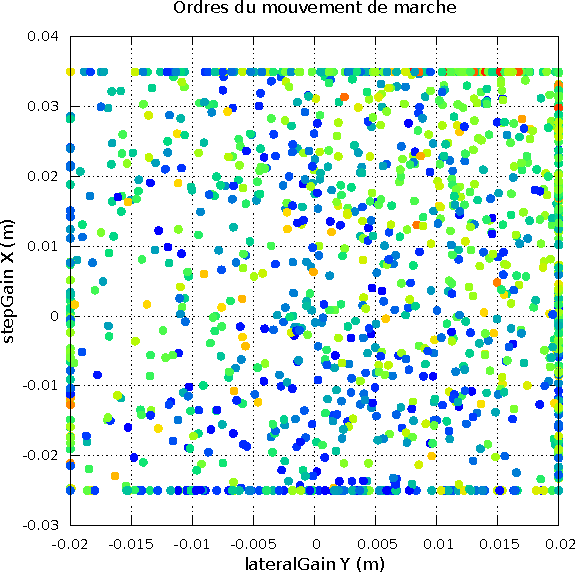
\includegraphics[type=pdf,ext=.pdf,read=.pdf,width=0.65\linewidth]{../plot/OdometryCMAES/walk_orders}
    \caption{\label{fig:odometry_cmaes_walk_orders} 
        Ordres envoyés au générateur de marche projetés sur le plan avance, latéral.
        Les ordres de toutes les séquences enregistrées ($25$) sont dessinés.
        On observe la dispersion dans l'espace d'action 
        dû au pilotage aléatoire de la marche pour par un mouvement brownien.
        La couleur du bleu au rouge représente le temps au sein de la séquence.
    }
\end{figure}

Sur le robot Sigmaban et sur l'herbe artificielle, un total de $25$ séquences de marche
ont été enregistrées.
D'une durée approximative de l'ordre de $15$~secondes, elles sont enregistrées à $100$ Hertz, 
contiennent entre $1222$ et $1877$ points (état des capteurs à un instant donné) 
et comptent entre $24$ et $38$ cycles de marche.
Un temps d'environ $30$ minutes et deux opérateurs ont été nécessaires 
pour l'acquisition de ses données.

La figure \ref{fig:odometry_cmaes_walk_orders} expose pour l'intégralité 
des séquences les ordres envoyés au générateur de la marche au cours du déplacement.
Cette figure est à comparer avec la figure \ref{fig:odometry_lwpr_logs} de l'étude précédente.
Grâce au pilotage automatique du robot par un processus aléatoire, la couverture 
de l'espace d'action est bien plus uniforme et présente moins de biais.
Cependant, on remarque que l'exploration aléatoire isotrope sur l'accélération combinée
au respect des bornes minimums et maximums a pour inconvénient d'accumuler les ordres 
sur les bordures de l'espace d'action.
Ce phénomène engendrant de forts ordres répétés sur plusieurs dimensions du contrôle
oblige à limiter les intervalles acceptables de vitesse de la marche 
afin de maintenir la stabilité du robot.

Dans la suite, ce faible nombre de données est utilisé pour le calcul 
des statistiques en se basant sur la méthode de validation 
croisée de Monte-Carlo.
L'ensemble des enregistrements est partitionné aléatoirement en deux groupes.
Un ensemble de validation de $5$ séquences et un ensemble
d'entrainement de $20$ séquences.
Après apprentissage, les modèles de correction sont évalués sur l'ensemble 
de validation.
Ce processus est répété $500$ fois puis la moyenne et la variance 
des évaluations sont calculées.

Lors de l'apprentissage, la précision du déplacement prédictif
du robot est évaluée par la fonction de récompense $\mathsf{fitness}()$ 
introduite précédemment.
Pour la validation et afin d'obtenir une grandeur interprétable, 
les poses d'arrivées des déplacements sont évaluées par leur distance 
cartésienne moyenne à la mesure expérimentale. 
L'orientation finale n'est alors pas considérée.\\

\begin{figure}[htb]
    \centerfloat
    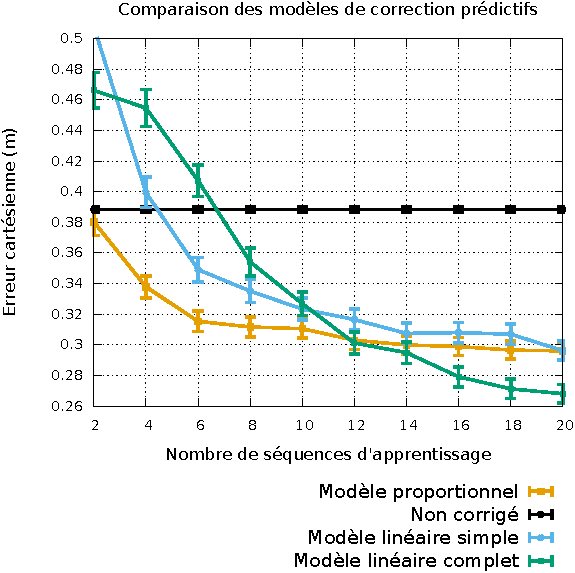
\includegraphics[type=pdf,ext=.pdf,read=.pdf,width=0.8\linewidth]{../plot/OdometryCMAES/convergenceOrders}
    \caption{\label{fig:odometry_cmaes_convergence_orders} 
        Convergence et comparaison de l'erreur cartésienne moyenne en position (prédictive)
        en fonction du nombre d'enregistrements utilisés pour l'apprentissage.
        Les trois modèles linéaires de corrections sont comparés à la prédiction
        de l'odométrie sans correction.
        Les marges de confiance à $95\%$ sont représentées.
    }
\end{figure}

L'optimisation CMA-ES est réalisée avec les méta paramètres suivants :
\begin{itemize}
    \item Nombre maximum d'itérations : $1000$
    \item Nombre de redémarrages : $3$
    \item Taille de la population : $50$
\end{itemize}
Grâce à l'implémentation multi-threadée de la bibliothèque \textit{libcmaes} en C++ et
de la non utilisation du modèle géométrique,
le temps d'optimisation hors ligne d'une correction à partir 
des séquences d'entrainement se situe aux alentours de la seconde.

Le graphique \ref{fig:odometry_cmaes_convergence_orders} présente les précisions
de prédiction des différents modèles de correction
en faisant varier le nombre de séquences utilisés pour leur entrainement.
Les commentaires suivants peuvent être faits :
\begin{itemize}
    \item Tout d'abord, tous les modèles de correction 
        même simples permettent d'améliorer la précision 
        de l'odométrie prédictive.
        L'erreur moyenne de prédiction de base étant 
        de $0.39$~m.
    \item Comme attendu, la convergence est d'autant plus lente
        que le nombre de paramètres du modèle est élevé.
        Un plus grand nombre de séquences d'apprentissage est alors nécessaire.
        Il ne faut que environ $10$ séquences pour identifier le modèle
        proportionnel alors $14$ et $20$ séquences sont respectivement
        nécessaires à la convergence des modèles linéaires simple et complet.
    \item La précision du modèle linéaire simple est équivalente à celle
        du modèle purement proportionnel (erreur de $0.30$~m).
        La différence entre les deux tient dans les termes de décalages 
        constants du modèle linéaire simple.
        En réalité, le mouvement de marche utilisé est déjà en partie 
        manuellement calibré dans l'axe avant arrière.
        Un terme de compensation (ajouté à l'ordre \textit{stepGain}) permet
        de garantir que le robot ne se déplace pas quand un ordre de déplacement 
        neutre lui est donné.
        La valeur de cette compensation\footnote{Cette compensation est importante. 
        Les erreurs d'asservissement des moteurs ainsi que la position du centre de masse 
        du robot sur l'axe avant arrière suffisent à faire avancer ou reculer le robot 
        même si l'ordre de marcher sur place lui est donné.} vaut $-0.08$~m.
        Les autres dimensions latérales et en rotation souffrent 
        peu de ce problème, ce qui explique la faible différence entre
        les deux modèles.
    \item Le modèle linéaire complet, prenant en compte les corrélations croisées 
        entre les ordres de marche, est le plus performant avec 
        $0.27$~m d'erreur moyenne.
        Cependant, le nombre de séquence de déplacement nécessaire à son entrainement 
        est important ; les $20$ séquences ne semblent qu'à peine suffisantes.
        En effet sur la figure \ref{fig:odometry_cmaes_convergence_orders},
        la courbe verte même avec $20$ séquences d'apprentissage ne forme pas
        un plateau et semble encore pouvoir légèrement descendre.
    \item Si l'on ne dispose que d'une dizaine d'enregistrements, le modèle 
        proportionnel est alors le meilleur choix.\\
\end{itemize}

En se basant sur le modèle linéaire complet et avec $20$ séquences d'entrainement, 
la précision de l'odométrie prédictive est de l'ordre de $0.27$~m d'erreur sur la position 
cartésienne après environs $30$ cycles de marche (soit $60$ pas).
Soit une erreur de prédiction divisée par $1.4$ grâce à la correction.
Pour comparaison, l'étude précédente employant le système de capture 
de mouvements externe et dans des conditions similaires 
(herbe artificielle, marche en boucle ouverte) accumulait environ $0.30$~m d'erreur moyenne
(voir la figure \ref{fig:odometry_lwpr_compare}).
Ces deux valeurs sont significativement semblables.
Sans correction, on obtient une erreur moyenne de l'ordre de $0.39$~m alors
que l'étude précédente faisait état dans les mêmes conditions d'une erreur moyenne
d'environ $0.60$~m avec un intervalle de confiance plus large.

Cet écart peut s'expliquer de deux manières.
Premièrement, la plateforme robotique a subit d'importantes modifications 
mécaniques et logicielles entre les deux expérimentations.
Il est possible que le changement du type de servomoteurs (Dynamixel RX vers MX)
et le doublement de la fréquence de mise à jour bas niveau aient
réduit les perturbations non systématiques de la marche.
Deuxièmement, une autre explication se trouve peut être dans les
différences d'ordres de marche entre les deux expérimentations.
Avec un pilotage automatique et aléatoire, le robot tend à faire 
plus de boucles et moins de trajectoires en lignes droites qu'avec
le pilotage manuel.
Le robot s'éloigne moins en moyenne du point de départ et
l'erreur cartésienne est ainsi statistiquement plus faible.
Il parait donc difficile de véritablement comparer précisément 
les résultats des deux études.\\

\begin{figure}[htb]
    \centerfloat
    \begin{subfigure}{0.4\paperwidth}
        \centering
        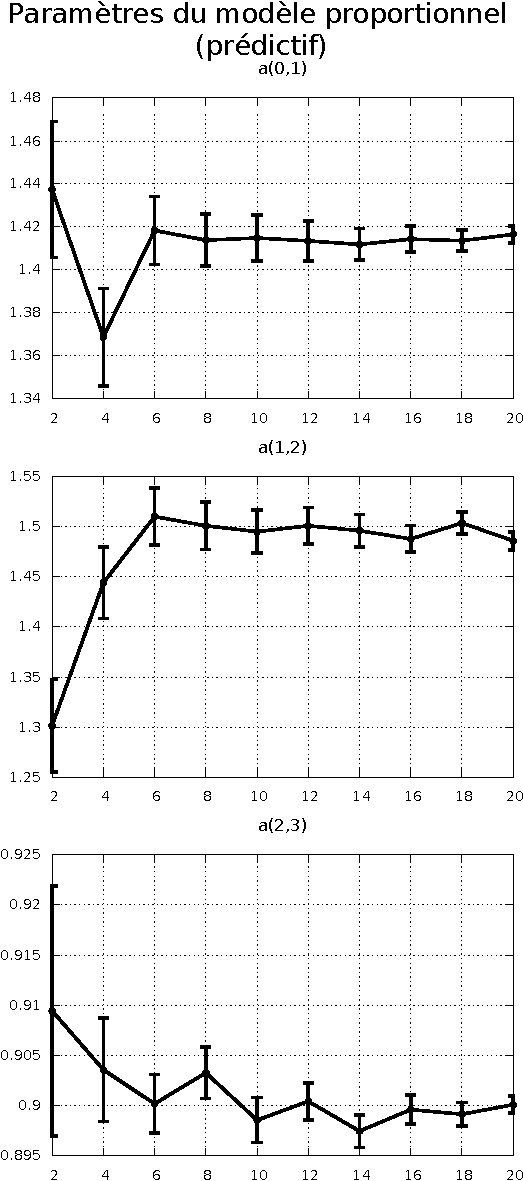
\includegraphics[type=pdf,ext=.pdf,read=.pdf,width=0.7\linewidth]{../plot/OdometryCMAES/parametersPropOrders}
    \end{subfigure}
    \begin{subfigure}{0.4\paperwidth}
        \centering
        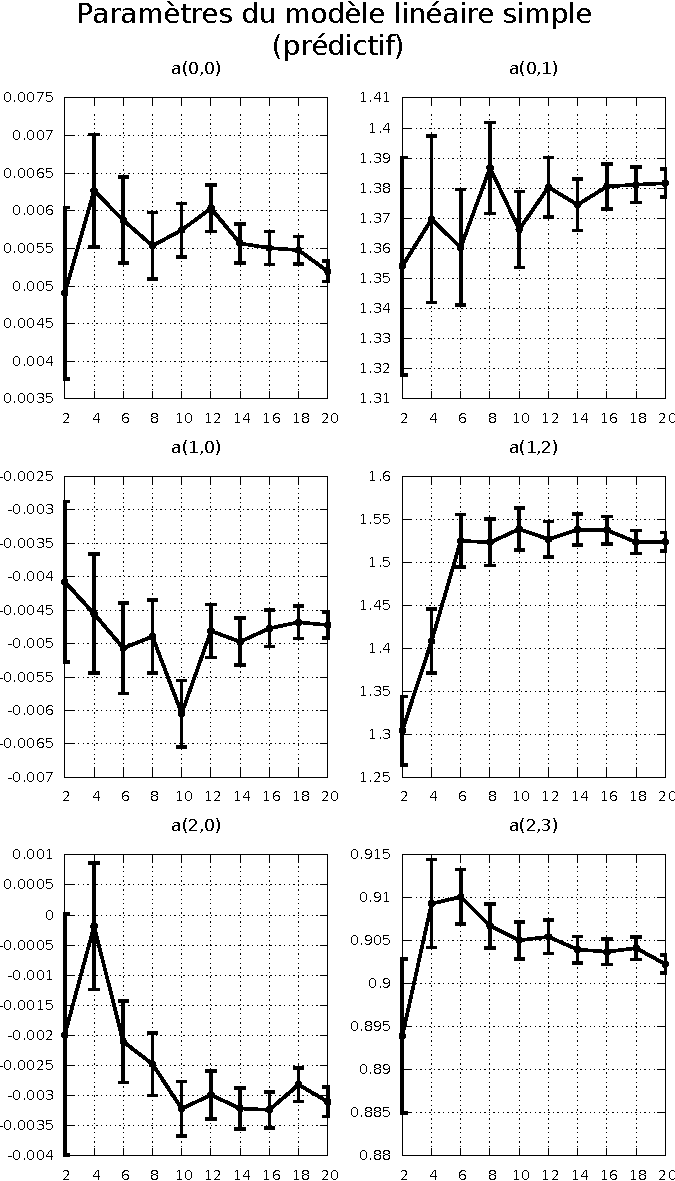
\includegraphics[type=pdf,ext=.pdf,read=.pdf,width=0.9\linewidth]{../plot/OdometryCMAES/parametersSimpleOrders}
    \end{subfigure}
    \caption{\label{fig:odometry_cmaes_parameters_prop_simple_orders} 
        Convergence des valeurs moyennes des $3$ et $6$ paramètres des modèles proportionnel 
        et linéaire simple (prédictifs) en fonction du nombre de séquences utilisées pour l'apprentissage.
        Les marges de confiance à $95\%$ sont représentées.
    }
\end{figure}
\begin{figure}[htb]
    \centerfloat
    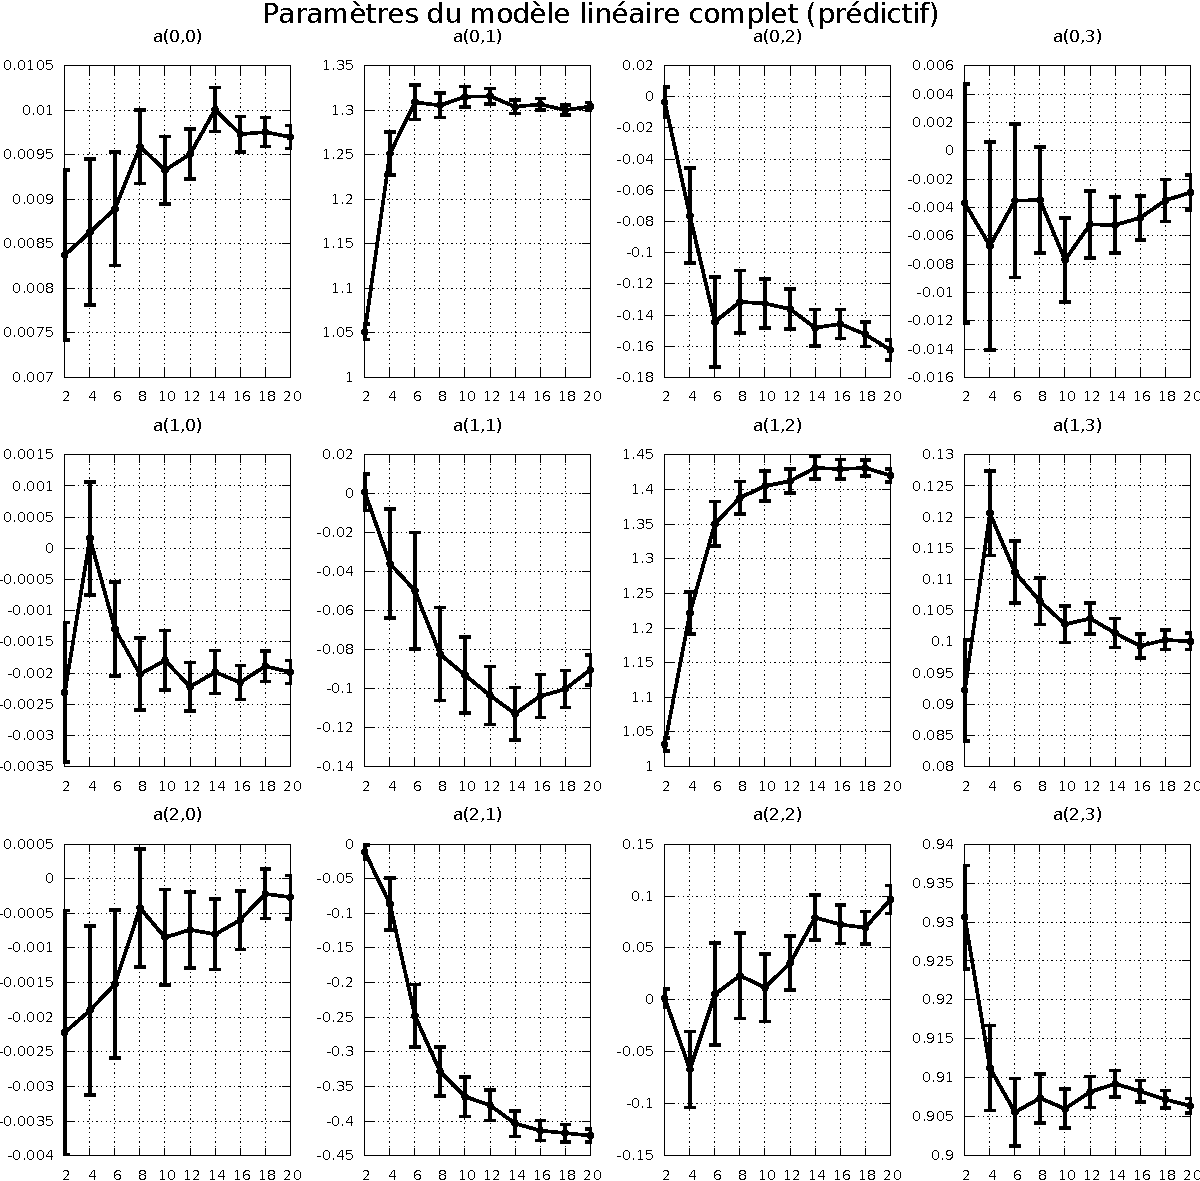
\includegraphics[type=pdf,ext=.pdf,read=.pdf,width=0.9\linewidth]{../plot/OdometryCMAES/parametersFullOrders}
    \caption{\label{fig:odometry_cmaes_parameters_full_orders} 
        Convergence des valeurs moyennes des $12$ paramètres du modèle linéaire complet (prédictif)
        en fonction du nombre de séquences utilisées pour l'apprentissage.
        Les marges de confiance à $95\%$ sont représentées.
    }
\end{figure}

Les deux graphiques \ref{fig:odometry_cmaes_parameters_prop_simple_orders} et 
\ref{fig:odometry_cmaes_parameters_full_orders} montrent la valeur moyenne et les marges de confiance
des différents paramètres après optimisation pour chacun des trois modèles linéaires en
fonction du nombre de séquences utilisées pour l'entrainement.
Ces graphiques inspirent les commentaires suivants :
\begin{itemize}
    \item Les coefficients proportionnels aux déplacements 
        avants et latéraux $a_{0,1},a_{1,2}$ sont à chaque fois entre $1.2$ et $1.6$. 
        L'odométrie prédictive sans correction sous-estime bien les déplacements
        en translation.
    \item A contrario, le coefficient proportionnel aux rotations $a_{2,3}$ est aux
        alentours de $0.9$. Ainsi, sans correction, le déplacement prédictif surestime 
        les rotations.
    \item Les valeurs des coefficients de compensation statiques $a_{0,0},a_{1,0},a_{2,0}$ 
        restent faibles car le mouvement de marche est déjà manuellement calibré 
        dans l'axe avant arrière.
    \item Comme remarqué sur les corrélations de l'étude précédente 
        (voir les graphiques \ref{fig:odometry_lwpr_function_goal}), les coefficients
        croisés $a_{1,1},a_{2,1},a_{0,2},a_{2,2},a_{1,3}$ du modèle linéaire complet 
        ont un impact significatif.
        Par exemple, les pas chassés ont une influence sur la translation 
        vers l'avant mais pas les rotations.
    \item Les marges de confiance des paramètres se resserrent avec l'augmentation
        du nombre des séquences d'entrainements.
        Ceci dénote une certaine robustesse des paramètres aux partitionnements aléatoires
        de l'ensemble d'apprentissage.
        Si les variances des paramètres avaient été trop élevées, cela aurait été
        une indication de surapprentissage.
    \item La convergence et le resserrement des marges de confiance est plus
        prononcés pour les coefficients proportionnels, responsables de la plus 
        grande part de la correction.\\
\end{itemize}

\begin{figure}[htb]
    \centerfloat
    \begin{subfigure}{0.28\paperwidth}
        \centering
        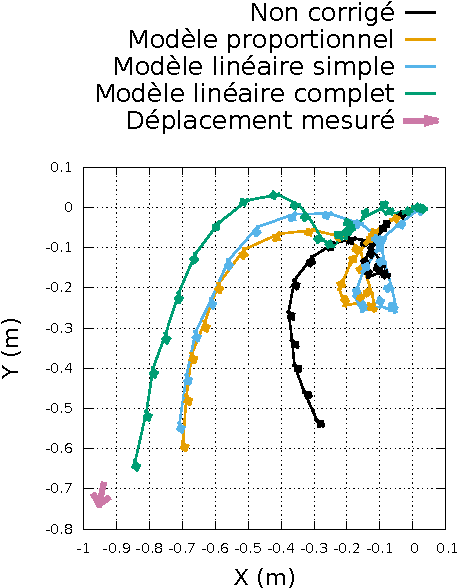
\includegraphics[type=pdf,ext=.pdf,read=.pdf,width=1.0\linewidth]{../plot/OdometryCMAES/ordersTraj1}
    \end{subfigure}
    \begin{subfigure}{0.28\paperwidth}
        \centering
        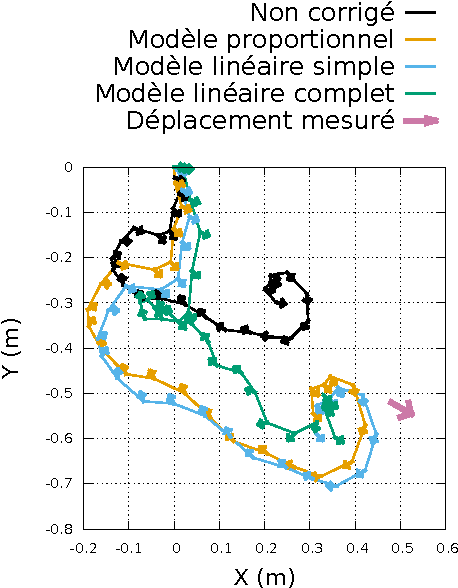
\includegraphics[type=pdf,ext=.pdf,read=.pdf,width=1.0\linewidth]{../plot/OdometryCMAES/ordersTraj2}
    \end{subfigure}
    \begin{subfigure}{0.28\paperwidth}
        \centering
        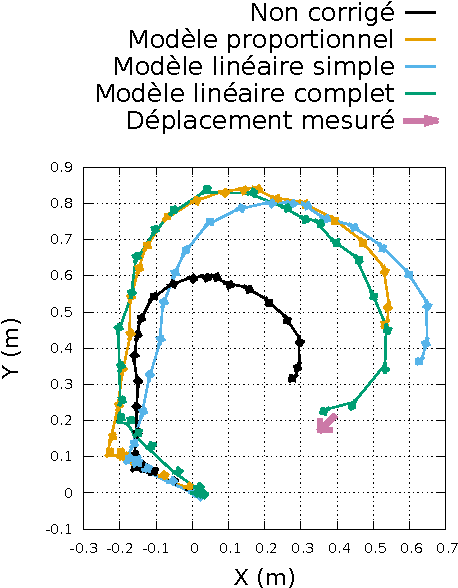
\includegraphics[type=pdf,ext=.pdf,read=.pdf,width=1.0\linewidth]{../plot/OdometryCMAES/ordersTraj3}
    \end{subfigure}
    \newline
    \begin{subfigure}{0.28\paperwidth}
        \centering
        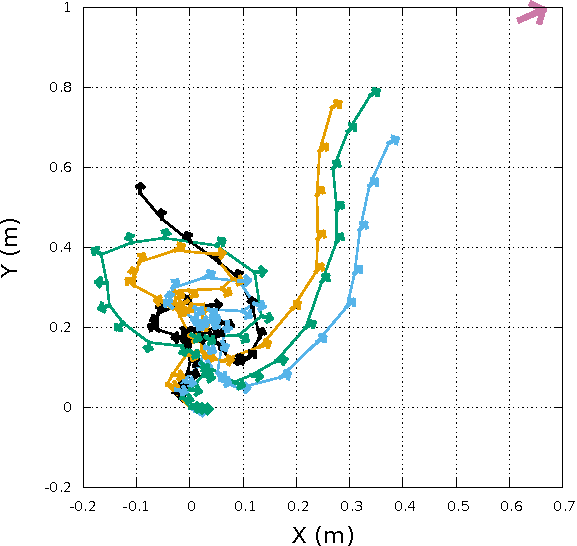
\includegraphics[type=pdf,ext=.pdf,read=.pdf,width=1.0\linewidth]{../plot/OdometryCMAES/ordersTraj4}
    \end{subfigure}
    \begin{subfigure}{0.28\paperwidth}
        \centering
        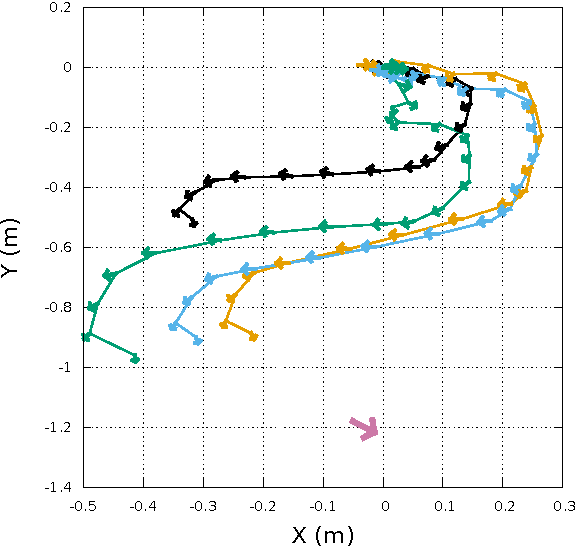
\includegraphics[type=pdf,ext=.pdf,read=.pdf,width=1.0\linewidth]{../plot/OdometryCMAES/ordersTraj5}
    \end{subfigure}
    \begin{subfigure}{0.28\paperwidth}
        \centering
        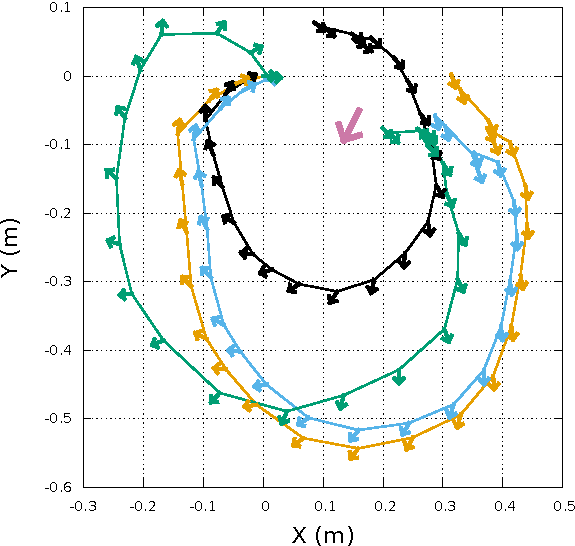
\includegraphics[type=pdf,ext=.pdf,read=.pdf,width=1.0\linewidth]{../plot/OdometryCMAES/ordersTraj6}
    \end{subfigure}
    \newline
    \begin{subfigure}{0.28\paperwidth}
        \centering
        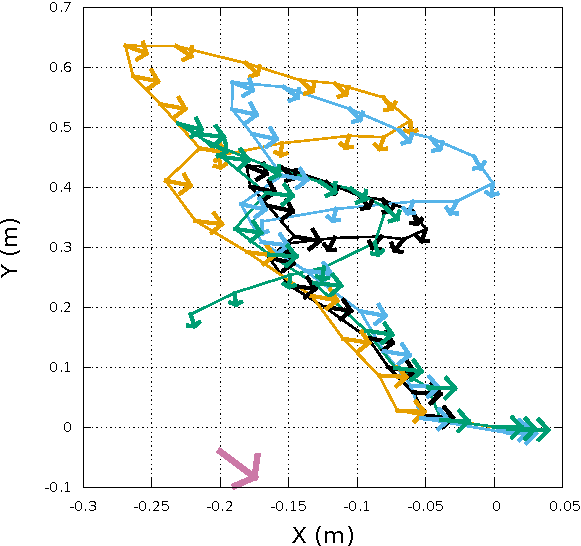
\includegraphics[type=pdf,ext=.pdf,read=.pdf,width=1.0\linewidth]{../plot/OdometryCMAES/ordersTraj7}
    \end{subfigure}
    \begin{subfigure}{0.28\paperwidth}
        \centering
        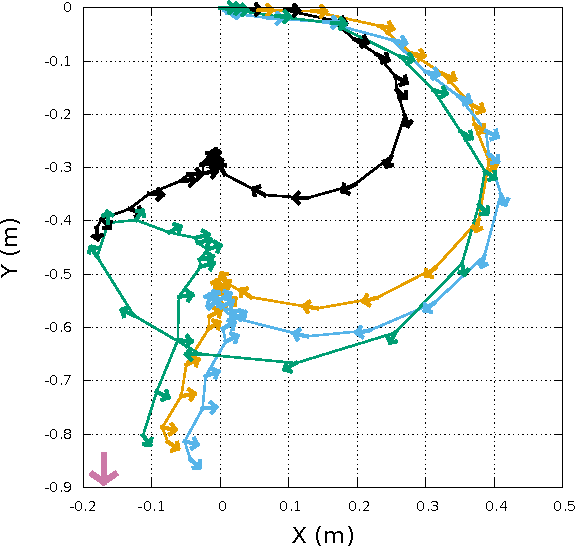
\includegraphics[type=pdf,ext=.pdf,read=.pdf,width=1.0\linewidth]{../plot/OdometryCMAES/ordersTraj8}
    \end{subfigure}
    \begin{subfigure}{0.28\paperwidth}
        \centering
        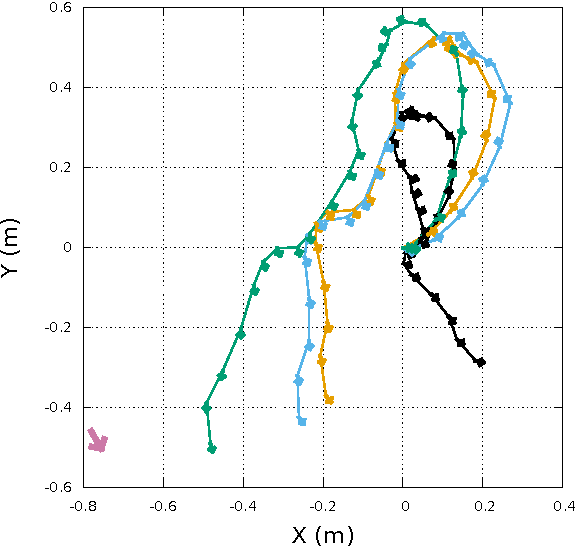
\includegraphics[type=pdf,ext=.pdf,read=.pdf,width=1.0\linewidth]{../plot/OdometryCMAES/ordersTraj9}
    \end{subfigure}
    \caption{\label{fig:odometry_cmaes_trajs_orders} 
        Comparaison sur neuf des séquences enregistrées de l'odométrie prédictive non
        corrigée et corrigée par les trois modèles linéaires après calibration.
        La pose finale mesurée est également représentée.
        Chaque point le long des trajectoires correspond à la pose prédictive du robot 
        au début de chaque cycle de marche.
        La pose de départ est centrée sur zéro.
    }
\end{figure}

Pour finir, la figure \ref{fig:odometry_cmaes_trajs_orders} illustre les trajectoires
simulées avec les différents modèles de correction sur $9$ des $25$ 
séquences enregistrées.\\

Pour l'apprentissage de la politique MDP et dans la suite, 
les déplacements du robot sont prédits et corrigés grâce 
au modèle linéaire complet.
Les $12$ paramètres du modèle sont ceux optimisés avec les $20$ séquences d'apprentissage.
Plus précisément, les valeurs choisies sont les moyennes
sur les $500$ ensembles d'apprentissage aléatoirement testés 
(représentés à la figure \ref{fig:odometry_cmaes_parameters_full_orders}).

\subsection{Odométrie proprioceptive}

À partir des mêmes données, les modèles de correction de l'odométrie proprioceptive 
peuvent également être construits.
Le graphique de convergence des erreurs moyennes (\ref{fig:odometry_cmaes_convergence_reads}),
de convergence des paramètres (\ref{fig:odometry_cmaes_parameters_prop_simple_reads}, 
\ref{fig:odometry_cmaes_parameters_full_reads}) et l'illustration des trajectoires 
du robot selon les différents modèles (\ref{fig:odometry_cmaes_trajs_reads})
peuvent être consultés en annexe à la section \ref{sec:odometry_cmaes_read_plots}.

Toujours avec $20$ séquences d'entrainement, et après une trentaine de cycles de marche, 
le modèle linéaire complet atteint une erreur cartésienne moyenne d'environ $0.11$~m 
alors que sans correction, l'erreur est de $0.21$~m.
Pour comparaison avec l'étude précédente, la correction se basant sur LWPR parvient
à une erreur moyenne de $0.17$~m contre $0.25$~m sans correction.

\subsection{Expérimentations et résultats du contrôle de l'approche}

Dans la suite, les trois politiques de contrôle suivantes sont
comparées sur le problème de l'approche de la balle.
\begin{description}
    \item[\textit{Expert}] : il s'agit de la politique implémentée manuellement 
        par une machine à états. Ses paramètres ont été ajustés à la main par 
        expérimentation du robot réel.
    \item[\textit{CMA-ES}] : c'est la même politique que \textit{\textbf{Expert}} mais ses paramètres 
        sont optimisés automatiquement grâce à la simulation du déplacement du robot 
        et à l'algorithme en boite noire CMA-ES.
    \item[\textit{RFPI}] : cette politique représentée sous la forme d'une forêt d'arbres 
        de régressions est générée par l'algorithme de résolution de MDP continus RFPI.
\end{description}
À chaque fois, les deux capacités de locomotion sont testées. 
La marche normale omnidirectionnelle et un mouvement quasiment non omnidirectionnel
amputé d'une grande partie de ses pas chassés.\\

\subsubsection{En simulation}

Dans un premier temps, les différentes politiques de contrôle
sont comparées en simulation (en se basant sur les déplacements corrigés).
Le tableau \ref{tab:odometry_cmaes_results_sim} présente 
le score moyen évaluant la performance des politiques dans chacun des cas.
Ce score est la moyenne de $10000$ approches
de la balle, à chaque fois évaluée par le critère défini précédemment 
(section \ref{sec:odometry_cmaes_fitness}).
Pour rappel, ce score correspond au nombre moyen de cycles de marche
nécessaire pour atteindre la zone de tir.\\

\begin{table}[h]
    \caption{
        \label{tab:odometry_cmaes_results_sim}Scores moyens 
        en simulation pour les différentes politiques}
    \centering
    \begin{tabular}{|l|c|c|c|}
        \hline
            & \textit{Expert} & \textit{CMA-ES} & \textit{RFPI} \\
        \hline
        Marche omnidirectionnelle     & 31.84      & 14.90  & 11.88      \\
        Marche quasiment non omnidirectionnelle   & 44.12      & 36.18  & 15.97 \\
        \hline
    \end{tabular}
\end{table}

Dans les deux cas omnidirectionnel et non omnidirectionnel, les politiques 
optimisées automatiquement \textit{CMA-ES} et \textit{RFPI} surpassent 
la politique manuelle.
Il s'avère donc bien que les paramètres de la politique experte 
ajustés manuellement sont loin d'être optimaux.
En pratique, il est en effet délicat de régler à la main les gains de l'asservissement 
afin que l'approche soit performante non pas sur une situation particulaire 
mais sur toutes les situations.
Sans critère quantitatif, le bon compromis est très difficile à atteindre.

Comme attendue, la politique \textit{Experte} n'est pas efficace dans le cas
quasiment non omnidirectionnel. De même, la politique optimisée \textit{CMA-ES}
est un peu meilleure mais sa forme fixée s'appuie nécessairement sur les pas chassés.
A contrario, la politique \textit{RFPI} s'adapte aux deux capacités de locomotion
car sa forme n'est pas imposée a priori.

\subsubsection{Sur le robot Sigmaban}

\begin{figure}[htb]
    \centerfloat
    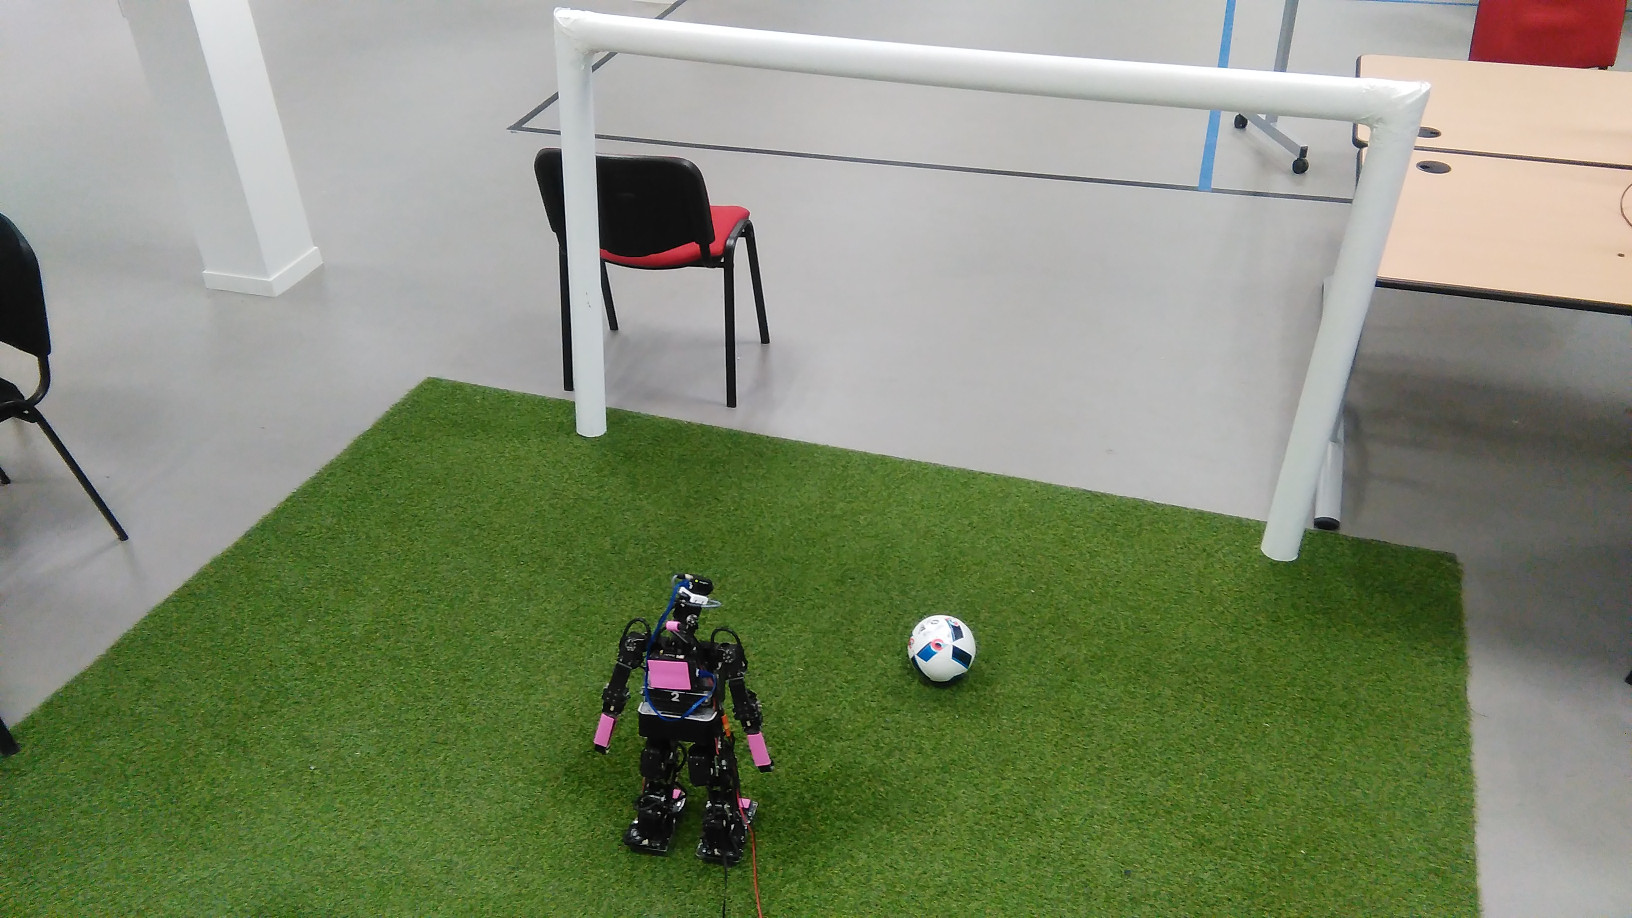
\includegraphics[width=1.0\linewidth]{../media/odometry_cmaes_setup.jpg}
    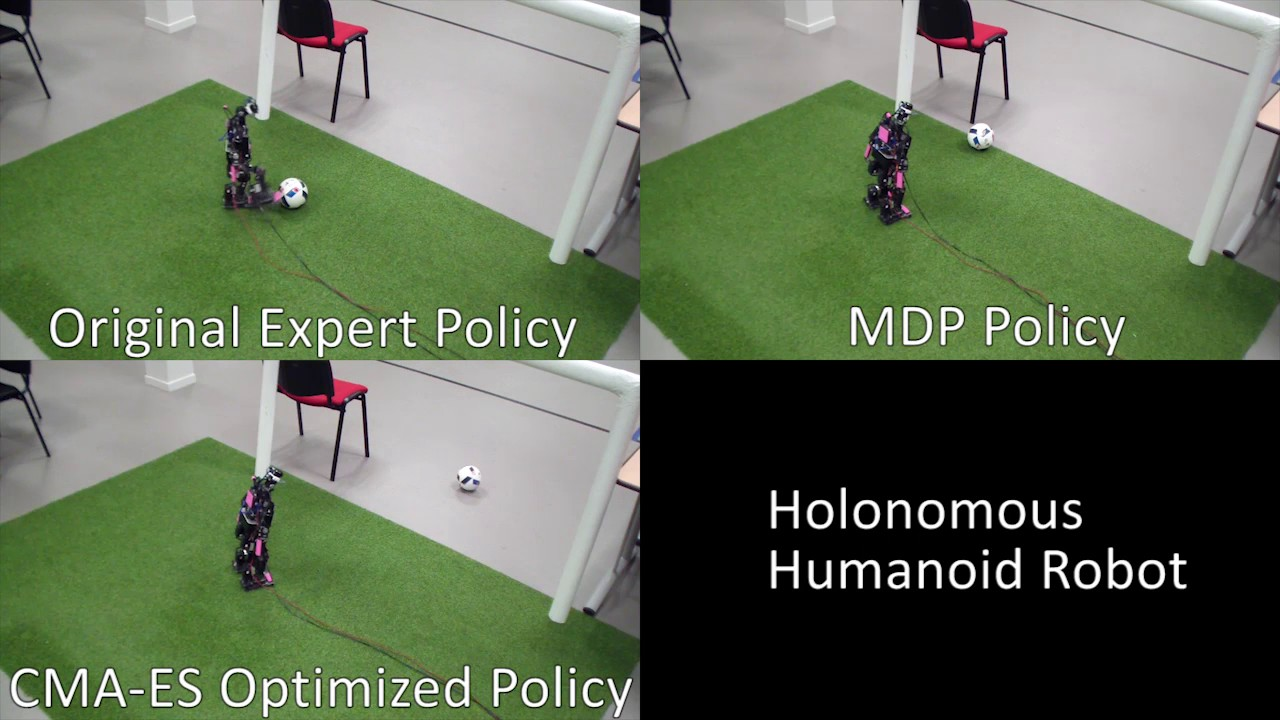
\includegraphics[width=1.0\linewidth]{../media/odometry_cmaes_setup2.jpg}
    \caption{\label{fig:odometry_cmaes_setup} 
        Photos du dispositif expérimental.
    }
\end{figure}

\begin{table}[htb]
    \caption{\label{tab:odometry_cmaes_results_real}Temps moyens en secondes pour se positionner 
        avant de tirer la balle}
    \centering
    \begin{tabular}{|l|c|c|c|}
        \hline
            & \textit{Expert} & \textit{CMA-ES} & \textit{RFPI} \\
        \hline
        Marche omnidirectionnelle   & 19.98      & 13.72  & 11.45      \\
        Marche quasiment non omnidirectionelle & 48.14      & 25.69  & 18.81 \\
        \hline
    \end{tabular}
\end{table}

\begin{figure}[htb]
    \centerfloat
    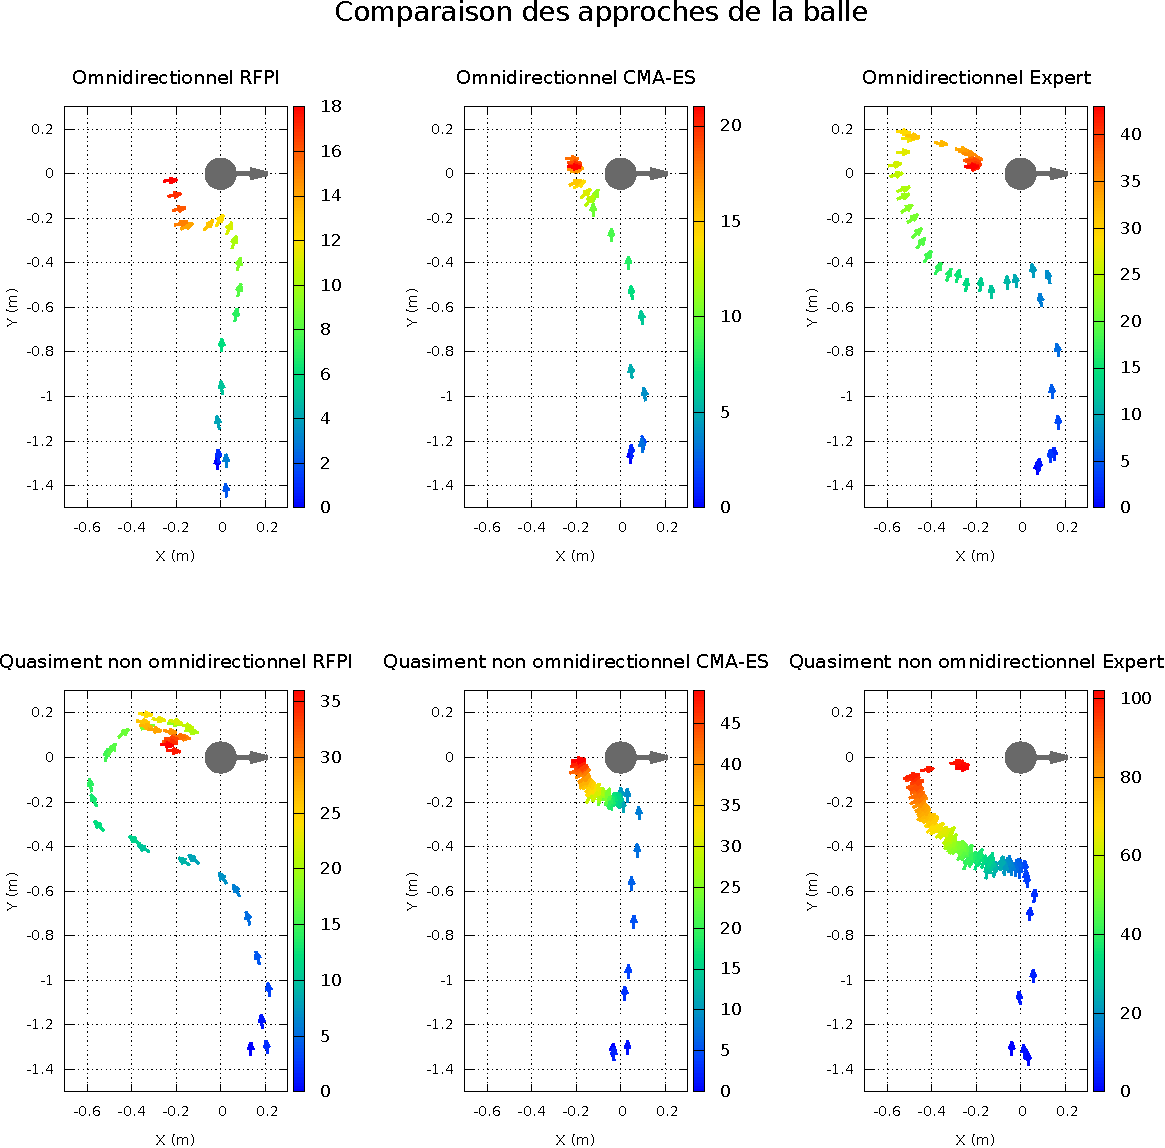
\includegraphics[type=pdf,ext=.pdf,read=.pdf,width=1.3\linewidth]{../plot/OdometryCMAES/robotTrajs}
    \caption{\label{fig:odometry_cmaes_robottrajs} 
        Comparaison des différentes politiques d'approche de la balle
        sur le robot réel Sigmaban.
        Les trajectoires sont mesurées par l'odométrie proprioceptive du robot.
        Chaque flèche représente la pose du robot à un cycle donné de marche.
        La couleur correspond au numéro du cycle de marche du bleu (pose de départ)
        au rouge (pose d'arrivée).
    }
\end{figure}

La vidéo présentant ces expérimentations peut être trouvée 
à l'adresse suivante :
\url{https://youtu.be/PNA-rpNKfsY}\\

Le robot Sigmaban est ici placé sur de l'herbe artificielle avec pour 
objectif de tirer dans la balle face aux buts 
(illustré à la figure \ref{fig:odometry_cmaes_setup}).
La balle utilisée est une petite balle blanche conforme au règlement de la RoboCup 2016.
Le module de vision du robot est spécialement adapté\footnote{Afin d'augmenter 
au maximum la fréquence de détection de la balle, la détection des buts ainsi 
que le module de localisation employés lors des matchs de football robotique sont désactivés.}
pour ne détecter que la balle à une fréquence d'environ $25$ Hertz.
La position relative de la balle dans le repère égocentrique du
robot est calculée au travers du modèle géométrique direct. 
Un filtre passe bas est également appliqué pour lisser la position de la balle.
La direction de tir est fournie manuellement au robot relativement à
son orientation initiale avant le début de chaque approche.
Le robot suit l'évolution de son orientation grâce à l'intégration
des gyromètres de sa centrale inertielle.\\

Chacune des trois politiques (\textit{Experte}, \textit{CMA-ES}, \textit{RFPI})
sur chacune des deux locomotions (omnidirectionnel et quasiment non omnidirectionnel) sont
testées sur le robot réel $12$ fois.
Soit un total de $72$ séquences d'approche de la balle.
Le produit cartésien des conditions suivantes est testé :
\begin{itemize}
    \item La balle est initialement placée à $1$ et $0.5$ mètre du robot. 
    \item La direction de tir dans le repère initial du robot est de $0$ et $180$ degrés.
    \item La balle est initialement placée devant, sur la gauche et sur le droite du robot.
\end{itemize}

À chaque fois, le temps nécessaire au robot pour se placer puis se stabiliser 
devant la balle dans la zone de tir est mesurée.
Les moyennes de ces temps sont reportées sur le tableau \ref{tab:odometry_cmaes_results_real}.\\

Pour terminer, le graphique \ref{fig:odometry_cmaes_robottrajs} illustre 
le comportement des différentes politiques sur le robot réel.
À noter que les trajectoires représentées ne sont pas les trajectoires réelles 
mais les trajectoires estimées par l'odométrie proprioceptive (non corrigée) du robot.
L'échelle de couleur permet de connaitre à chaque fois le nombre de cycles de marche
de l'approche.

\subsection{Discussion et conclusion}

Entre cette étude et les travaux précédant se basant sur 
la capture de mouvement, la plateforme robotique a évoluée.
Ces améliorations mécaniques, électroniques et logicielles imposent 
une certaine prudence dans la comparaison précise des résultats.
À ceci, il faut ajouter la différence de méthode d'enregistrement 
des données entre le pilotage manuel à la manette et une exploration 
aléatoire automatique.
La mesure manuelle du déplacement ne nécessite aucun dispositif
lourd à mettre en place et peut être appliquée dans le contexte
opérationnel d'une compétition RoboCup.
Mais contrairement à l'étude précédente, le temps humain
requis par la mesure limite fortement la quantité de données
pouvant être enregistrée.

Comme le nombre de séquences total est faible, il n'est pas envisageable
de les séparer en un ensemble d'entrainement et un ensemble de validation
suffisamment grand pour être significatif.
Les statistiques estimées sont donc également sujettes à caution.
La méthode de validation croisée de Monte-Carlos choisie a pour intérêt
de sélectionner uniformément les séquences dans l'ensemble des $25 \choose 20$ configurations 
de validations possibles.
Ce choix tend à privilégier une faible variance mais une moyenne plus biaisée.
Ainsi, les marges de confiances calculées ici ne peuvent réellement 
être comparées qu'au sein de cette étude.

Malgré ces précautions, la tendance semble néanmoins montrer que les précisions
de l'odométrie prédictive et proprioceptive après optimisation par CMA-ES 
sont similaires à celles obtenues avec LWPR.
Il faut souligner la différence très importante de quantité d'information disponible aux deux méthodes.
Ici, seulement une vingtaine de séquences de marche et la mesure de la pose finale est nécessaire
alors que l'intégralité des déplacements entre chaque pas était précédemment utilisé.
Ceci tend à valider la forme linéaire du modèle de correction.

À noter que d'autres modèles linéaires intégrant l'influence des ordres 
de la marche au cycle précédant (effets inertiels) ont été expérimentés.
Nécessitant plus de paramètres et donc plus de séquences d'entrainement, 
leur convergence n'a pas été suffisante avec les données disponibles.
Notons également que le développement d'un système de localisation par reconnaissance 
de balises visuelles facilement transportables a été commencé par l'équipe.
Un tel système permettrait de mesurer automatiquement le déplacement final du robot
et allègerait l'effort humain d'enregistrement des données.\\

Il manque dans l'expérimentation des politiques de contrôle la validation
de l'utilité réelle de la calibration de l'odométrie prédictive.
Le bon fonctionnement de l'algorithme RFPI pour l'apprentissage de la politique 
de contrôle MDP est prouvé.
Cependant, il n'est pas en l'état démontré que le modèle de correction
influence l'efficacité de la politique dans l'approche de la balle. 
Peut être que l'asservissement du mouvement est suffisant pour garantir
la précision du déplacement.
Il faudrait pouvoir tester sur le robot réel une politique de contrôle générée 
à partir d'une simulation du déplacement du robot non corrigée et mesurer 
sa performance.
Ceci constitue le principal défaut de ces expérimentations.

La politique de contrôle basée sur le formalisme MDP surpasse
en simulation ainsi que sur le robot réel les autres politiques.
Ceci tient en son adaptabilité au problème puisque la forme du 
contrôle n'est pas préalablement fixée.
Néanmoins, dans le contexte normale de la marche omnidirectionnelle, 
la différence de performance entre la politique MDP et la politique 
experte optimisée par CMA-ES n'est pas très élevée.
De plus, les temps de calculs sont très différents.
Il faut moins de $30$ secondes pour optimiser l'approche experte 
à l'aide de la simulation des déplacements du robot alors 
que plus d'une heure est nécessaire pour la construction
de la politique MDP.

Si la stricte optimalité n'est pas nécessaire et si la forme d'une politique
experte paramétrée est facilement implémentable manuellement, 
l'optimisation en boite noire de ses paramètres est une méthode à considérer.

